\documentclass[usenames,dvipsnames,t]{beamer}
\usetheme{Rochester}

\usepackage{tikz}
\usepackage[utf8]{inputenc}
\usepackage{setspace}
\usepackage{bbding}
\usepackage{microtype}

%Information to be included in the title page:
\title{Implementing the Genesis Chain Selection Rule}
\author{Edsko de Vries}
\institute{Well-Typed}
\date{November 2020}

\begin{document}

\frame{\titlepage}

%%%%%%%%%%%%%%%%%%%%%%%%%%%%%%%%%%%%%%%%%%%%%%%%%%%%%%%%%%%%%%%%%%%%%%%%%%%%%%%%

\begin{frame}
\frametitle{The Genesis Rule}

\begin{alertblock}{Genesis chain selection rule}
A candidate chain is preferred over our current chain if

\begin{itemize}
\item The intersection between the candidate chain and our chain is \textbf{no
more than $k$} blocks back, and the candidate chain is strictly \textbf{longer}
than our chain.

\item If the intersection \emph{is} \textbf{more than $k$} blocks back, and the
candidate chain is \textbf{denser} (contains more blocks) than our chain in
a region of $s$ slots starting at the intersection.
\end{itemize}
\end{alertblock}

\end{frame}

%%%%%%%%%%%%%%%%%%%%%%%%%%%%%%%%%%%%%%%%%%%%%%%%%%%%%%%%%%%%%%%%%%%%%%%%%%%%%%%%

\begin{frame}
\frametitle{The Genesis Rule}

\begin{alertblock}{Alternative genesis rule}
A candidate chain is preferred over our current chain if

\begin{itemize}
\item The intersection between the candidate chain and our chain is
\textbf{at least $s$ slots} back, and the candidate chain is denser in a window
of $s$ slots at the intersection, or

\item The intersection between the candidate chain and our chain is \textbf{no
more than $k$ blocks} back, and the candidate chain is strictly \textbf{longer}
than our chain.
\end{itemize}

\end{alertblock}

\end{frame}

%%%%%%%%%%%%%%%%%%%%%%%%%%%%%%%%%%%%%%%%%%%%%%%%%%%%%%%%%%%%%%%%%%%%%%%%%%%%%%%%

\begin{frame}
\frametitle{Fundamental Assumptions within the Consensus Layer}

%%%%%%%%%%%%%%%%%%%%%%%%%%%%%%%%%%%%%%%%

\begin{onlyenv}<1>

\begin{alertblock}{Invariant}
We never roll back more than $k$ blocks.
\end{alertblock}

This invariant is used to

\begin{itemize}
\item \textbf{Organise on-disk and in-memory block and ledger storage}: blocks older
than $k$ are stored in the \emph{immutable} database, the remainder in the
\emph{volatile} database.
\item \textbf{Guarantee efficient block validation}: we have access to the $k$
most recent ledger states
\item \textbf{Bound memory usage for tracking peers}: we need to track at most $k + 1$
blocks per upstream peer to be able to decide if we prefer their chain over
ours (apply the longest chain rule)
\item \dots
\end{itemize}

\end{onlyenv}

%%%%%%%%%%%%%%%%%%%%%%%%%%%%%%%%%%%%%%%%

\begin{onlyenv}<2>
\begin{alertblock}{Invariant}
We never switch to a shorter chain.
\end{alertblock}

\pause

Without this invariant, the previous invariant (never roll back
more than $k$ blocks) is not very useful.

\begin{itemize}
\item If we \emph{could} switch to a shorter chain but continue to support a
rollback of $k$, the \emph{effective} maximum rollback is infinite.
\item We would need efficient access to \emph{all} past ledger states.
\item We would have to move blocks \emph{back} from the immutable database to the volatile database.
\item \dots
\end{itemize}
\end{onlyenv}

%%%%%%%%%%%%%%%%%%%%%%%%%%%%%%%%%%%%%%%%

\begin{onlyenv}<3>

\begin{alertblock}{Invariant}
The strict extension of a chain is always preferred over that chain.
\end{alertblock}

\begin{itemize}
\item Used to make some local chain selection decisions.
\item (I \emph{think} this one is compatible with Genesis.)
\end{itemize}

\end{onlyenv}

\end{frame}

%%%%%%%%%%%%%%%%%%%%%%%%%%%%%%%%%%%%%%%%%%%%%%%%%%%%%%%%%%%%%%%%%%%%%%%%%%%%%%%%

\begin{frame}{Towards an Alternative}

\begin{center}
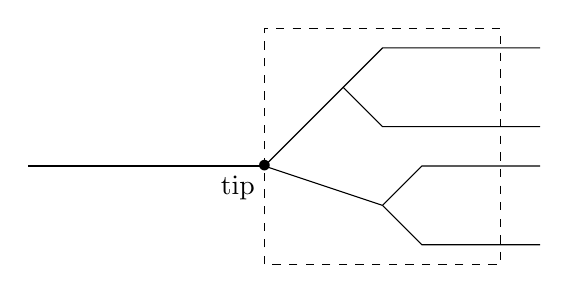
\begin{tikzpicture}
\path (0, 0) coordinate (tip) node{$\bullet$} node[below left]{tip};
\draw (tip) + (-3,0) -- (tip);
\onslide<2->{\draw (tip) -- ++(1.0,  1.0) coordinate (ab);}
\onslide<3->{\draw (tip) -- ++(1.5, -0.5) coordinate (cd);}
\onslide<4->{\draw (ab) -- ++(0.5,  0.5) -- ++(2.0, 0);}
\onslide<5->{\draw (ab) -- ++(0.5, -0.5) -- ++(2.0, 0);}
\onslide<6->{\draw (cd) -- ++(0.5,  0.5) -- ++(1.5, 0);}
\onslide<7->{\draw (cd) -- ++(0.5, -0.5) -- ++(1.5, 0);}
\onslide<8->{\draw [dashed] (tip) -- ++(0, 1.75) -- ++(3, 0) -- ++(0, -3) -- ++(-3, 0) -- cycle;}
\end{tikzpicture}
\end{center}

\end{frame}

%%%%%%%%%%%%%%%%%%%%%%%%%%%%%%%%%%%%%%%%%%%%%%%%%%%%%%%%%%%%%%%%%%%%%%%%%%%%%%%%

\begin{frame}
\frametitle{Towards an Alternative}

\begin{onlyenv}<1>

\begin{alertblock}{Key Idea: Delay the decision}
Rather than adopting chain $A$ as soon as we see it,
and later switch to chain $B$ (possibly incurring a large rollback), \emph{wait}:
don't adopt \emph{either} $A$ \emph{or} $B$ until we know which one we want.
\end{alertblock}

Assumptions:

\begin{itemize}
\item We can guarantee that we see (a representative sample of) all chains
in the network. An attacker \textbf{can't eclipse} us.
\item We can \textbf{detect when} we should delay because the genesis condition
might apply. \\
(We will come back to this.) \\
\end{itemize}

\end{onlyenv}

\end{frame}

%%%%%%%%%%%%%%%%%%%%%%%%%%%%%%%%%%%%%%%%%%%%%%%%%%%%%%%%%%%%%%%%%%%%%%%%%%%%%%%%

\begin{frame}

\frametitle<1-4>{Choosing between forks: at genesis}
\frametitle<5>{Choosing between forks: general case}

\begin{center}
\begin{tikzpicture}
\path (0, 0) coordinate (tip) node{$\bullet$} node[below left]{tip};
\draw (tip) -- ++(1.0,  1.0) coordinate (ab) node{$\bullet$} node[above left]{$ab$};
\draw [dotted] (tip) -- ++(1.5, -0.5) coordinate (cd);
\draw (ab) -- ++(0.5,  0.5) -- ++(2.0, 0) coordinate(A) node[right]{$A$};
\draw (ab) -- ++(0.5, -0.5) -- ++(2.0, 0) node[right]{$B$};
\draw [dotted] (cd) -- ++(0.5,  0.5) -- ++(1.5, 0) node[right]{$C$};
\draw [dotted] (cd) -- ++(0.5, -0.5) -- ++(1.5, 0) node[right]{$D$};
\draw [dashed]
     (tip)
  -- ++(0, 1.75)
  -- ++(3, 0)
  -- ++(0, -3)
  -- ++(-3, 0) node[pos=0.5, below]{$\underbrace{\hspace{3cm}}_{\text{$s$ slots}}$}
  -- cycle;
\path (tip) -- (A) node[pos=0.5, above=1cm]{$\overbrace{\hspace{3.5cm}}^{\text{$> k$ blocks}}$};

%%%%%%%%%%%%%%%%%%%%%%%%%%%%%%%%%%%%%%%%

\onslide<1-2>{\draw (tip) -- ++(1.5, -0.5) node{$\bullet$};}
\onslide<1-2>{\draw (cd) -- ++(0.5,  0.5) -- ++(1.5, 0);}
\onslide<1-2>{\draw (cd) node[below left]{$cd$} -- ++(0.5, -0.5) -- ++(1.5, 0);}
\onslide<2-5>{\draw [red, very thick] (tip) -- (ab) -- ++(0.5,  0.5) -- ++(1.5, 0) ;}
\onslide<5>{\draw (tip) + (-3,0) node{$\bullet$} -- (tip);}
\end{tikzpicture}
\end{center}

\vspace{-1em}

\onslide<4-5>{
\begin{alertblock}{Committing}
By assumption, we have seen all relevant chains. We will \emph{never} be
interested in $C$ or $D$, so we can disconnect from them.
\end{alertblock}
}

\end{frame}

%%%%%%%%%%%%%%%%%%%%%%%%%%%%%%%%%%%%%%%%%%%%%%%%%%%%%%%%%%%%%%%%%%%%%%%%%%%%%%%%

\begin{frame}

\frametitle<1-4>{Common prefix: at genesis}
\frametitle<5>{Common prefix: general case}

\begin{center}
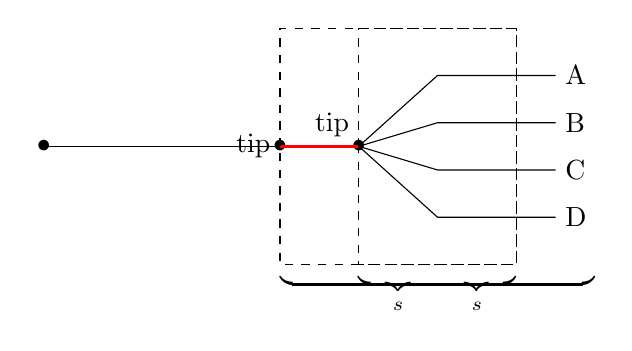
\begin{tikzpicture}
\path (0, 0) coordinate (tip) node{$\bullet$};
\draw (tip) -- ++(1.0,  0.0) coordinate (branch) node{$\bullet$};
\draw (branch) -- ++(1.0,  0.9) -- ++ (1.5, 0) node[right]{A};
\draw (branch) -- ++(1.0,  0.3) -- ++ (1.5, 0) node[right]{B};
\draw (branch) -- ++(1.0, -0.3) -- ++ (1.5, 0) node[right]{C};
\draw (branch) -- ++(1.0, -0.9) -- ++ (1.5, 0) node[right]{D};

%%%%%%%%%%%%%%%%%%%%%%%%%%%%%%%%%%%%%%%%

\onslide<1-2>{\node [left] at (tip) {tip};}
\onslide<2>{\draw [red, very thick] (tip) -- ++(1.0,  0.0);}
\onslide<3-5>{\node [above left] at (branch) {tip};}
\onslide<1-2>{\draw [dashed]
     (tip)
  -- ++(0, 1.5)
  -- ++(3, 0)
  -- ++(0, -3)
  -- ++(-3, 0) node[pos=0.5, below]{$\underbrace{\hspace{3cm}}_s$}
  -- cycle;}
\onslide<3-5>{\draw [dashed]
     (branch)
  -- ++(0, 1.5)
  -- ++(2, 0)
  -- ++(0, -3)
  -- ++(-2, 0)  node[pos=0.25, below]{$\underbrace{\hspace{3cm}}_s$}
  -- cycle;}
\onslide<5>{\draw (tip) + (-3,0) node{$\bullet$} -- (tip);}

\end{tikzpicture}
\end{center}

\onslide<4-5>{
\begin{alertblock}{Committing}
By assumption, we have seen all relevant chains. They all share a common prefix.
We can \emph{commit to} the blocks on that common prefix: they will never
be rolled back.
\end{alertblock}
}

\end{frame}

%%%%%%%%%%%%%%%%%%%%%%%%%%%%%%%%%%%%%%%%%%%%%%%%%%%%%%%%%%%%%%%%%%%%%%%%%%%%%%%%

\begin{frame}

\frametitle{Insufficient peers}

\begin{center}
\begin{tikzpicture}[yscale=0.75]
\path (0, 0) -- (6,0) node[left] {\color{red} \XSolidBrush};
\path (0, 0) coordinate (tip) node{$\bullet$} node[below left]{tip};
\draw (tip) -- ++(1.0,  1.0) coordinate (ab) node{$\bullet$} node[above left]{$ab$};
\draw (tip) -- ++(1.5, -0.5) coordinate (cd);
\draw (ab) -- ++(0.5,  0.5) -- ++(2.0, 0) node[right]{$A$};
\draw (ab) -- ++(0.5, -0.5) -- ++(2.0, 0) node[right]{$B$};
\draw (cd) -- ++(0.5,  0.5) -- ++(1.5, 0) node[right]{$C$};
\path (cd) -- ++(0.5, -0.5) -- ++(1.5, 0) coordinate (D);
\path (tip) -- (A) node[pos=0.5, above=0.6cm]{$\overbrace{\hspace{3.5cm}}^{\text{$> k$ blocks}}$};

\draw [dashed]
     (tip)
  -- ++(0, 1.75)
  -- ++(3, 0)
  -- ++(0, -3)
  -- ++(-3, 0) node[pos=0.5, below]{$\underbrace{\hspace{3cm}}_s$}
  -- cycle;
\draw [dotted] (D) -- ++(-2.5,0) -- ++(-0.25,0.25);

\draw [red, very thick] (tip) -- (ab) -- ++(0.5,  0.5) -- ++(1.5, 0) ;
\draw (tip) + (-3,0) node{$\bullet$} -- (tip);
\end{tikzpicture}
\end{center}

\begin{center}
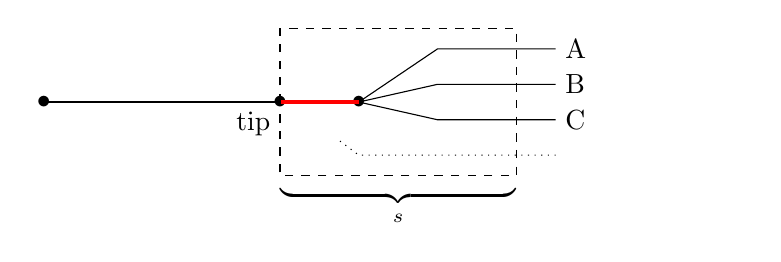
\begin{tikzpicture}[yscale=0.75]
\path (0, 0) -- (6,0) node[left] {\color{red} \XSolidBrush};
\path (0, 0) coordinate (tip) node{$\bullet$};
\draw (tip) -- ++(1.0,  0.0) coordinate (branch) node{$\bullet$};
\draw (branch) -- ++(1.0,  0.9) -- ++ (1.5, 0) node[right]{A};
\draw (branch) -- ++(1.0,  0.3) -- ++ (1.5, 0) node[right]{B};
\draw (branch) -- ++(1.0, -0.3) -- ++ (1.5, 0) node[right]{C};
\path (branch) -- ++(1.0, -0.9) -- ++ (1.5, 0) coordinate(D);

\draw [dotted] (D) -- ++(-2.5,0) -- ++(-0.25,0.25);
\node [below left] at (tip) {tip};
\draw [red, very thick] (tip) -- ++(1.0,  0.0);
\draw [dashed]
     (tip)
  -- ++(0, 1.25)
  -- ++(3, 0)
  -- ++(0, -2.5)
  -- ++(-3, 0) node[pos=0.5, below]{$\underbrace{\hspace{3cm}}_s$}
  -- cycle;
\draw (tip) + (-3,0) node{$\bullet$} -- (tip);

\end{tikzpicture}
\end{center}

\end{frame}

%%%%%%%%%%%%%%%%%%%%%%%%%%%%%%%%%%%%%%%%%%%%%%%%%%%%%%%%%%%%%%%%%%%%%%%%%%%%%%%%

\begin{frame}

\frametitle{Insufficient blocks}

\begin{center}
\begin{tikzpicture}[yscale=0.75]
\path (0, 0) -- (6,0) node[left] {\color{red} \XSolidBrush};
\path (0, 0) coordinate (tip) node{$\bullet$} node[below left]{tip};
\draw (tip) -- ++(1.0,  1.0) coordinate (ab) node{$\bullet$} node[above left]{$ab$};
\draw (tip) -- ++(1.5, -0.5) coordinate (cd);
\draw (ab) -- ++(0.5,  0.5) -- ++(2.0, 0) node[right]{$A$};
\draw (ab) -- ++(0.5, -0.5) -- ++(2.0, 0) node[right]{$B$};
\draw (cd) -- ++(0.5,  0.5) -- ++(1.5, 0) node[right]{$C$};
\draw (cd) -- ++(0.5, -0.5) node{$\bullet$} node[right]{$D$};
\path (tip) -- (A) node[pos=0.5, above=0.6cm]{$\overbrace{\hspace{3.5cm}}^{\text{$> k$ blocks}}$};

\draw [dashed]
     (tip)
  -- ++(0, 1.75)
  -- ++(3, 0)
  -- ++(0, -3.25)
  -- ++(-3, 0) node[pos=0.5, below]{$\underbrace{\hspace{3cm}}_s$}
  -- cycle;

\draw [red, very thick] (tip) -- (ab) -- ++(0.5,  0.5) -- ++(1.5, 0) ;
\draw (tip) + (-3,0) node{$\bullet$} -- (tip);
\end{tikzpicture}
\end{center}

\begin{center}
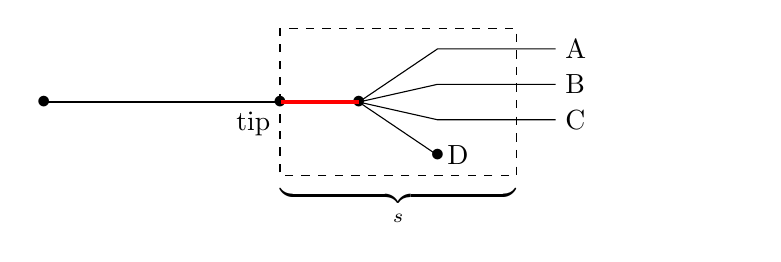
\begin{tikzpicture}[yscale=0.75]
\path (0, 0) -- (6,0) node[left] {\color{ForestGreen} \CheckmarkBold};
\path (0, 0) coordinate (tip) node{$\bullet$};
\draw (tip) -- ++(1.0,  0.0) coordinate (branch) node{$\bullet$};
\draw (branch) -- ++(1.0,  0.9) -- ++ (1.5, 0) node[right]{A};
\draw (branch) -- ++(1.0,  0.3) -- ++ (1.5, 0) node[right]{B};
\draw (branch) -- ++(1.0, -0.3) -- ++ (1.5, 0) node[right]{C};
\draw (branch) -- ++(1.0, -0.9) node{$\bullet$} node[right]{D};

\node [below left] at (tip) {tip};
\draw [red, very thick] (tip) -- ++(1.0,  0.0);
\draw [dashed]
     (tip)
  -- ++(0, 1.25)
  -- ++(3, 0)
  -- ++(0, -2.5)
  -- ++(-3, 0) node[pos=0.5, below]{$\underbrace{\hspace{3cm}}_s$}
  -- cycle;
\draw (tip) + (-3,0) node{$\bullet$} -- (tip);

\end{tikzpicture}
\end{center}

\end{frame}

%%%%%%%%%%%%%%%%%%%%%%%%%%%%%%%%%%%%%%%%%%%%%%%%%%%%%%%%%%%%%%%%%%%%%%%%%%%%%%%%

\begin{frame}

\frametitle{Threshold for sufficient blocks}

\begin{center}
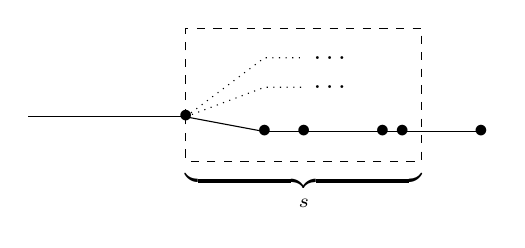
\begin{tikzpicture}[yscale=0.75]
\draw (0,0) -- (2,0) node{$\bullet$} coordinate (tip);
\draw [dotted] (tip) -- ++(1,1) -- ++ (0.5,0) node[right]{$\ldots$};
\draw [dotted] (tip) -- ++(1,0.5) -- ++ (0.5,0) node[right]{$\ldots$};
\draw (tip) -- ++(1,-0.25) node {$\bullet$} coordinate (a);
\onslide<2-6>{\draw (a) -- ++(0.5,  0) node {$\bullet$} coordinate (b);}
\onslide<3-6>{\draw (b) -- ++(1.0,  0) node {$\bullet$} coordinate (c);}
\onslide<4-6>{\draw (c) -- ++(0.25, 0) node {$\bullet$} coordinate (d);}
\onslide<5-6>{\draw (d) -- ++(1,    0) node {$\bullet$} coordinate (e);}
\draw [dashed]
     (tip)
  -- ++(0, 1.5)
  -- ++(3, 0)
  -- ++(0, -2.25)
  -- ++(-3, 0) node[pos=0.5, below]{$\underbrace{\hspace{3cm}}_s$}
  -- cycle;
\end{tikzpicture}
\end{center}

\onslide<6>{
\begin{alertblock}{Dealing with nodes that don't provide sufficient blocks}
As part of the protocol, nodes report their tip. Was optimisation, now becomes essential:

\begin{itemize}
\item Disconnect from nodes that report a chain shorter than $s$.
\item Timeout from nodes that report a chain longer than $s$ but don't send
us blocks (DoS attack).
\end{itemize}
\end{alertblock}
}

\end{frame}

%%%%%%%%%%%%%%%%%%%%%%%%%%%%%%%%%%%%%%%%%%%%%%%%%%%%%%%%%%%%%%%%%%%%%%%%%%%%%%%%

\begin{frame}

\frametitle{Detecting when to delay}

\begin{itemize}
\item \textbf{\alert{Cannot} apply density rule when we are closer than $s$ slots from the
wallclock slot.}
\\ (We would be unable to fill the window, by definition.)
\item \textbf{\alert{Don't need} to apply density rule when within $k = 2160$ blocks from
the wallclock slot.} [Handwavy] \\
(Too?) liberal rephrasing of Theorem 2 of the genesis paper.
\item \textbf{Always sound to delay chain selection} \\
(Unless \emph{really} near tip and we might have to forge a block) \\
\item Paper suggests $s = \frac{1}{4} (k/f)$ = 10,800 slots. \\
(I.e. $s \times f = \frac{1}{4}k = 540$ blocks on average.)
\end{itemize}

\begin{alertblock}{}
\textbf{Delay if more than $s$ slots from the wallclock.} \\
(If wallclock slot unknown,  must be more than $(3k/f) > s$ slots.)
\end{alertblock}

\end{frame}

%%%%%%%%%%%%%%%%%%%%%%%%%%%%%%%%%%%%%%%%%%%%%%%%%%%%%%%%%%%%%%%%%%%%%%%%%%%%%%%%

\begin{frame}

\frametitle{Generalising delay mode}

\begin{center}
\begin{tikzpicture}[yscale=0.75]
\path (0, 0) coordinate (tip) node{$\bullet$} node[below left]{tip};
\draw (tip) -- ++(1.0,  1.0) coordinate (ab) node{$\bullet$} node[above left]{$ab$};
\draw [dotted] (tip) -- ++(1.5, -0.5) coordinate (cd);
\draw (ab) -- ++(0.5,  0.5) -- ++(2.0, 0) coordinate(A) node[right]{$A$};
\draw (ab) -- ++(0.5, -0.5) -- ++(2.0, 0) node[right]{$B$};
\draw [dotted] (cd) -- ++(0.5,  0.5) -- ++(1.5, 0) node[right]{$C$};
\draw [dotted] (cd) -- ++(0.5, -0.5) -- ++(1.5, 0) node[right]{$D$};
\draw [dashed]
     (tip)
  -- ++(0, 1.75)
  -- ++(3, 0)
  -- ++(0, -3)
  -- ++(-3, 0) node[pos=0.5, below]{$\underbrace{\hspace{3cm}}_{\text{$s$ slots}}$}
  -- cycle;
\path (tip) -- (A) node[pos=0.5, above=0.7cm]{$\overbrace{\hspace{3.5cm}}^{\text{may be fewer than $k$ blocks}}$};

\draw (tip) -- ++(1.5, -0.5) node{$\bullet$};
\draw (cd) -- ++(0.5,  0.5) -- ++(1.5, 0);
\draw (cd) node[below left]{$cd$} -- ++(0.5, -0.5) -- ++(1.5, 0);
\draw [red, very thick] (tip) -- (ab) -- ++(0.5,  0.5) -- ++(1.5, 0) ;
\draw (tip) + (-3,0) node{$\bullet$} -- (tip);
\end{tikzpicture}
\end{center}

\vspace{-1em}

\begin{itemize}
\item \textbf{Cannot reliably detect} whether we have more than $k$ blocks \\
(node reports tip but we cannot verify)
\item \textbf{Can still apply genesis condition}, independent of \# blocks \\
(justified by alternative genesis rule)
\end{itemize}

\end{frame}

%%%%%%%%%%%%%%%%%%%%%%%%%%%%%%%%%%%%%%%%%%%%%%%%%%%%%%%%%%%%%%%%%%%%%%%%%%%%%%%%

\begin{frame}

\frametitle{Header/Body split: choosing between forks}

\begin{center}
\begin{tikzpicture}[yscale=0.75]
\path (0, 0) coordinate (tip) node{$\bullet$} node[below left]{tip};
\draw (tip) -- ++(1.0,  1.0) coordinate (ab) node{$\bullet$} node[above left]{$ab$};
\draw [dotted] (tip) -- ++(1.5, -0.5) coordinate (cd);
\draw (ab) -- ++(0.5,  0.5) -- ++(2.0, 0) coordinate(A) node[right]{$A$};
\draw (ab) -- ++(0.5, -0.5) -- ++(2.0, 0) node[right]{$B$};
\draw [dotted] (cd) -- ++(0.5,  0.5) -- ++(1.5, 0) node[right]{$C$};
\draw [dotted] (cd) -- ++(0.5, -0.5) -- ++(1.5, 0) node[right]{$D$};
\draw [dashed]
     (tip)
  -- ++(0, 1.75)
  -- ++(3, 0)
  -- ++(0, -3)
  -- ++(-3, 0) node[pos=0.5, below]{$\underbrace{\hspace{3cm}}_{\text{$s$ slots}}$}
  -- cycle;

\draw [red, very thick] (tip) -- (ab) -- ++(0.5,  0.5) -- ++(1.5, 0) ;
\draw (tip) + (-3,0) node{$\bullet$} -- (tip);
\end{tikzpicture}
\end{center}

\vspace{-1em}

\begin{itemize}
\item What if we find an invalid block on $A$ after discarding $C$, $D$?
\item Header validation justifies deciding before block validation.
\begin{minipage}{0.9\textwidth}
\tiny\linespread{0.5} Christian: ``Intuitively, right after the forking point, the lottery to elect slot leaders is still the same on both chains, and there, no adversarial chain can be denser.''
\end{minipage}
\item Header validation (as separate from block validation) critical. \\
{\small (So far was ``merely'' required to guard against DoS attacks.)}
\end{itemize}

\end{frame}

%%%%%%%%%%%%%%%%%%%%%%%%%%%%%%%%%%%%%%%%%%%%%%%%%%%%%%%%%%%%%%%%%%%%%%%%%%%%%%%%

\begin{frame}

\frametitle{Header/Body split: common prefix}

\begin{center}
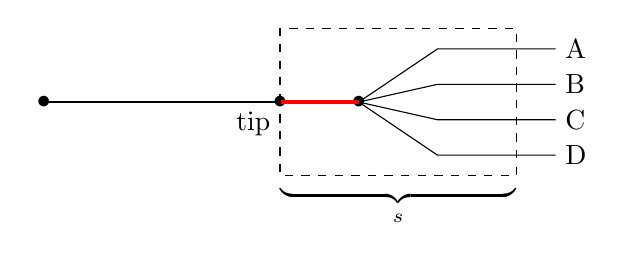
\begin{tikzpicture}[yscale=0.75]
\path (0, 0) coordinate (tip) node{$\bullet$};
\draw (tip) -- ++(1.0,  0.0) coordinate (branch) node{$\bullet$};
\draw (branch) -- ++(1.0,  0.9) -- ++ (1.5, 0) node[right]{A};
\draw (branch) -- ++(1.0,  0.3) -- ++ (1.5, 0) node[right]{B};
\draw (branch) -- ++(1.0, -0.3) -- ++ (1.5, 0) node[right]{C};
\draw (branch) -- ++(1.0, -0.9) -- ++ (1.5, 0) node[right]{D};

%%%%%%%%%%%%%%%%%%%%%%%%%%%%%%%%%%%%%%%%

\node [below left] at (tip) {tip};
\draw [red, very thick] (tip) -- ++(1.0,  0.0);
\draw [dashed]
     (tip)
  -- ++(0, 1.25)
  -- ++(3, 0)
  -- ++(0, -2.5)
  -- ++(-3, 0) node[pos=0.5, below]{$\underbrace{\hspace{3cm}}_s$}
  -- cycle;
\draw (tip) + (-3,0) node{$\bullet$} -- (tip);

\end{tikzpicture}
\end{center}

\begin{itemize}
\item Blocks from common prefix will be validated by chain database before adoption.
\item If found to be invalid, something went horribly wrong and we are eclipsed by
an attacker after all. Disconnect from all peers and start over.
\end{itemize}

\end{frame}

%%%%%%%%%%%%%%%%%%%%%%%%%%%%%%%%%%%%%%%%%%%%%%%%%%%%%%%%%%%%%%%%%%%%%%%%%%%%%%%%

\begin{frame}

\frametitle{Open questions}

\begin{itemize}
\item Assumption is that when we see $n$ peers, that gives us a representative sample of all chains in the network. Does that mean that after we discard some peers (not dense enough), we do not have have to look for more peers (apart from for performance reasons, perhaps)?
\item Detection of genesis mode OK?
\item Applying genesis condition even if fork closer than $k$ okay?
\item Concerns about invalid blocks with valid headers?
\item Anything else..?
\end{itemize}

\end{frame}

%%%%%%%%%%%%%%%%%%%%%%%%%%%%%%%%%%%%%%%%%%%%%%%%%%%%%%%%%%%%%%%%%%%%%%%%%%%%%%%%

\begin{frame}

\frametitle{Flip-flopping}

\begin{center}
\begin{tikzpicture}
\path (0, 0) coordinate (tip) node{$\bullet$} node[below left]{tip};
\draw (tip) -- ++(1.0,  0.5) -- ++(2.5, 0) coordinate(A) node[right]{$A$};
\draw (tip) -- ++(1.0, -0.5) -- ++(3.5, 0) coordinate(B) node[right]{$B$};
\draw [red, very thick] (tip) -- ++(1.0,  0.5) -- ++(2.0, 0);
\draw [dashed]
     (tip)
  -- ++(0, 0.75)
  -- ++(3, 0)
  -- ++(0, -1.5)
  -- ++(-3, 0) node[pos=0.5, below]{$\underbrace{\hspace{3cm}}_{\text{$s$ slots}}$}
  -- cycle;
\path (tip) -- (A) node[pos=0.5, above=0.5cm]{$\overbrace{\hspace{3.5cm}}^{\text{fewer than $k$ blocks}}$};
\path (tip) -- (B) node[pos=0.5, below=1.1cm]{$\underbrace{\hspace{4.5cm}}_{\text{more than $k$ blocks}}$};
\draw (tip) + (-3,0) node{$\bullet$} -- (tip);
\end{tikzpicture}
\end{center}

\pause

$A$ is preferred over $B$, and $B$ is preferred over $A$!


\end{frame}

\end{document}
